\documentclass{standalone}
\usepackage{tikz}
\usetikzlibrary{patterns, positioning}


\begin{document}
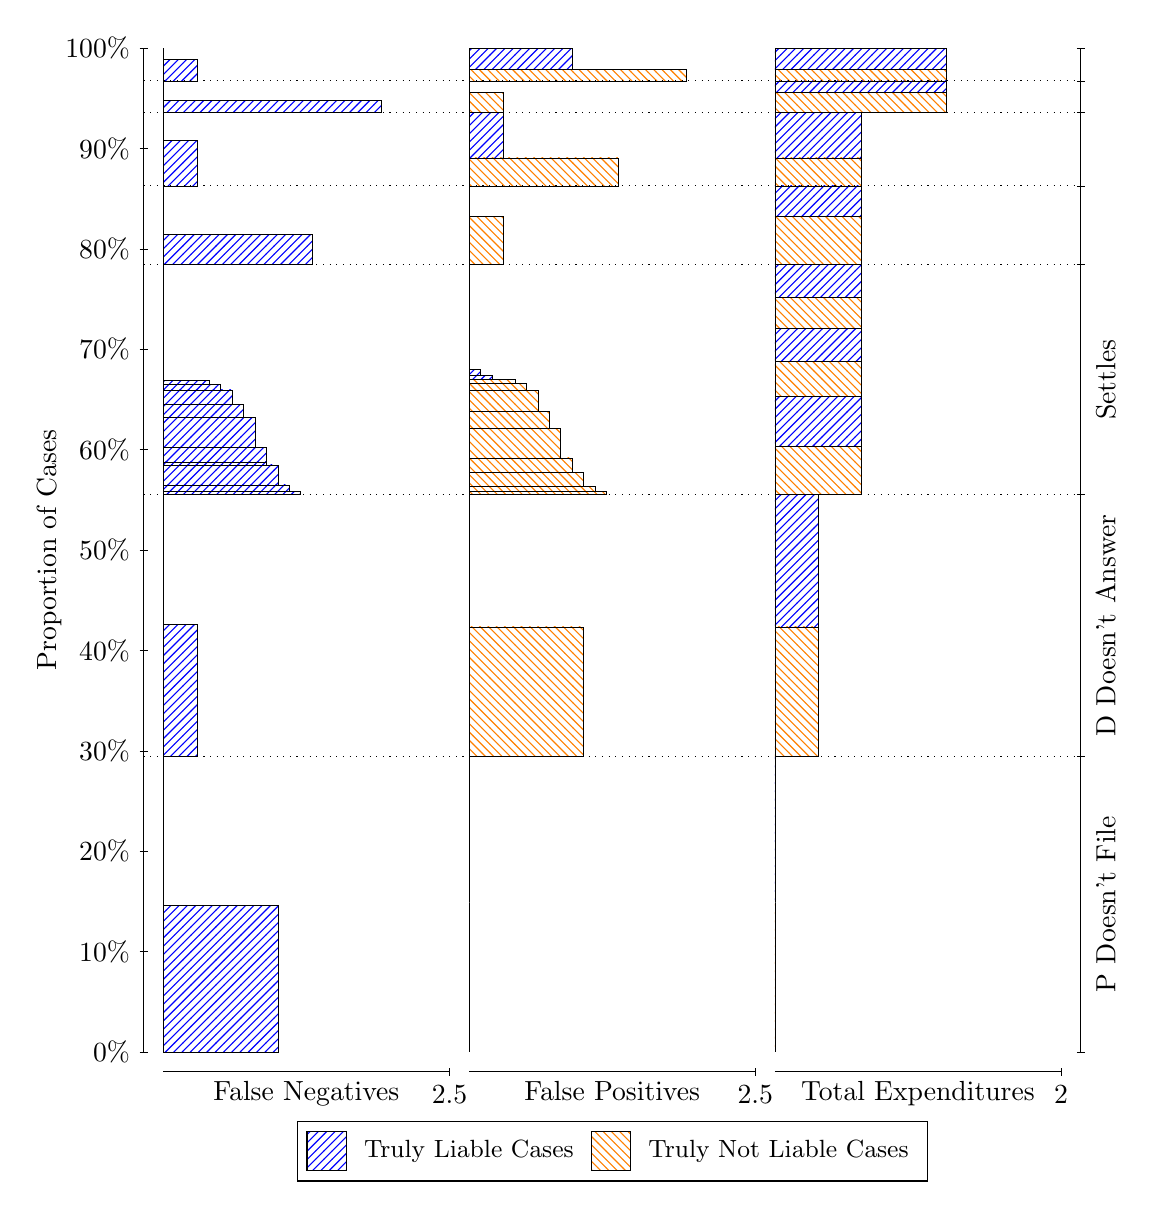
\begin{tikzpicture}
\draw[black, very thin] (1.5,1.75) -- (1.5,14.5);
\node[rotate=90, text=black, anchor=center] at (0.3, 8.125) {Proportion of Cases};
\draw[black, very thin] (1.45,1.75) -- (1.55,1.75);
\node[text=black, anchor=east] at (1.45, 1.75) {0\%};
\draw[black, very thin] (1.45,3.025) -- (1.55,3.025);
\node[text=black, anchor=east] at (1.45, 3.025) {10\%};
\draw[black, very thin] (1.45,4.3) -- (1.55,4.3);
\node[text=black, anchor=east] at (1.45, 4.3) {20\%};
\draw[black, very thin] (1.45,5.575) -- (1.55,5.575);
\node[text=black, anchor=east] at (1.45, 5.575) {30\%};
\draw[black, very thin] (1.45,6.85) -- (1.55,6.85);
\node[text=black, anchor=east] at (1.45, 6.85) {40\%};
\draw[black, very thin] (1.45,8.125) -- (1.55,8.125);
\node[text=black, anchor=east] at (1.45, 8.125) {50\%};
\draw[black, very thin] (1.45,9.4) -- (1.55,9.4);
\node[text=black, anchor=east] at (1.45, 9.4) {60\%};
\draw[black, very thin] (1.45,10.675) -- (1.55,10.675);
\node[text=black, anchor=east] at (1.45, 10.675) {70\%};
\draw[black, very thin] (1.45,11.95) -- (1.55,11.95);
\node[text=black, anchor=east] at (1.45, 11.95) {80\%};
\draw[black, very thin] (1.45,13.225) -- (1.55,13.225);
\node[text=black, anchor=east] at (1.45, 13.225) {90\%};
\draw[black, very thin] (1.45,14.5) -- (1.55,14.5);
\node[text=black, anchor=east] at (1.45, 14.5) {100\%};

\draw[black, very thin] (13.4,1.75) -- (13.4,14.5);
\draw[black, very thin] (13.35,1.75) -- (13.45,1.75);
\node[anchor=west] at (13.35, 1.75) {};
\draw[black, very thin] (13.35,5.5042) -- (13.45,5.5042);
\node[anchor=west] at (13.35, 5.5042) {};
\draw[black, very thin] (13.35,8.8283) -- (13.45,8.8283);
\node[anchor=west] at (13.35, 8.8283) {};
\draw[black, very thin] (13.35,11.748) -- (13.45,11.748);
\node[anchor=west] at (13.35, 11.748) {};
\draw[black, very thin] (13.35,12.75) -- (13.45,12.75);
\node[anchor=west] at (13.35, 12.75) {};
\draw[black, very thin] (13.35,13.678) -- (13.45,13.678);
\node[anchor=west] at (13.35, 13.678) {};
\draw[black, very thin] (13.35,14.084) -- (13.45,14.084);
\node[anchor=west] at (13.35, 14.084) {};
\draw[black, very thin] (13.35,14.5) -- (13.45,14.5);
\node[anchor=west] at (13.35, 14.5) {};

\draw[black, very thin, pattern color=blue, pattern=north east lines] (1.75,1.75) rectangle (3.2033,3.6071);
\draw[black, very thin, pattern color=orange, pattern=north west lines] (1.75,3.6071) rectangle (1.75,5.5042);
\draw[black, very thin, pattern color=blue, pattern=north east lines] (1.75,5.5042) rectangle (2.186,7.1833);
\draw[black, very thin, pattern color=orange, pattern=north west lines] (1.75,7.1833) rectangle (1.75,8.8283);
\draw[black, very thin, pattern color=blue, pattern=north east lines] (1.75,8.8283) rectangle (3.494,8.8734);
\draw[black, very thin, pattern color=blue, pattern=north east lines] (1.75,8.8734) rectangle (3.3487,8.9531);
\draw[black, very thin, pattern color=blue, pattern=north east lines] (1.75,8.9531) rectangle (3.2033,9.2052);
\draw[black, very thin, pattern color=blue, pattern=north east lines] (1.75,9.2052) rectangle (3.058,9.2427);
\draw[black, very thin, pattern color=blue, pattern=north east lines] (1.75,9.2427) rectangle (3.058,9.4284);
\draw[black, very thin, pattern color=blue, pattern=north east lines] (1.75,9.4284) rectangle (2.9127,9.8065);
\draw[black, very thin, pattern color=blue, pattern=north east lines] (1.75,9.8065) rectangle (2.7673,9.9789);
\draw[black, very thin, pattern color=blue, pattern=north east lines] (1.75,9.9789) rectangle (2.622,10.158);
\draw[black, very thin, pattern color=blue, pattern=north east lines] (1.75,10.158) rectangle (2.4767,10.232);
\draw[black, very thin, pattern color=blue, pattern=north east lines] (1.75,10.232) rectangle (2.3313,10.284);
\draw[black, very thin, pattern color=orange, pattern=north west lines] (1.75,10.284) rectangle (1.75,11.748);
\draw[black, very thin, pattern color=blue, pattern=north east lines] (1.75,11.748) rectangle (3.6393,12.138);
\draw[black, very thin, pattern color=orange, pattern=north west lines] (1.75,12.138) rectangle (1.75,12.75);
\draw[black, very thin, pattern color=blue, pattern=north east lines] (1.75,12.75) rectangle (2.186,13.323);
\draw[black, very thin, pattern color=orange, pattern=north west lines] (1.75,13.323) rectangle (1.75,13.678);
\draw[black, very thin, pattern color=blue, pattern=north east lines] (1.75,13.678) rectangle (4.5113,13.831);
\draw[black, very thin, pattern color=orange, pattern=north west lines] (1.75,13.831) rectangle (1.75,14.084);
\draw[black, very thin, pattern color=blue, pattern=north east lines] (1.75,14.084) rectangle (2.186,14.352);
\draw[black, very thin, pattern color=orange, pattern=north west lines] (1.75,14.352) rectangle (1.75,14.5);
\draw[black, very thin, pattern color=orange, pattern=north west lines] (5.6333,1.75) rectangle (5.6333,3.6471);
\draw[black, very thin, pattern color=blue, pattern=north east lines] (5.6333,3.6471) rectangle (5.6333,5.5042);
\draw[black, very thin, pattern color=orange, pattern=north west lines] (5.6333,5.5042) rectangle (7.0867,7.1493);
\draw[black, very thin, pattern color=blue, pattern=north east lines] (5.6333,7.1493) rectangle (5.6333,8.8283);
\draw[black, very thin, pattern color=orange, pattern=north west lines] (5.6333,8.8283) rectangle (7.3773,8.8713);
\draw[black, very thin, pattern color=orange, pattern=north west lines] (5.6333,8.8713) rectangle (7.232,8.9344);
\draw[black, very thin, pattern color=orange, pattern=north west lines] (5.6333,8.9344) rectangle (7.0867,9.1102);
\draw[black, very thin, pattern color=orange, pattern=north west lines] (5.6333,9.1102) rectangle (6.9413,9.2938);
\draw[black, very thin, pattern color=orange, pattern=north west lines] (5.6333,9.2938) rectangle (6.796,9.6726);
\draw[black, very thin, pattern color=orange, pattern=north west lines] (5.6333,9.6726) rectangle (6.6507,9.8822);
\draw[black, very thin, pattern color=orange, pattern=north west lines] (5.6333,9.8822) rectangle (6.5053,10.152);
\draw[black, very thin, pattern color=orange, pattern=north west lines] (5.6333,10.152) rectangle (6.36,10.243);
\draw[black, very thin, pattern color=orange, pattern=north west lines] (5.6333,10.243) rectangle (6.2147,10.293);
\draw[black, very thin, pattern color=blue, pattern=north east lines] (5.6333,10.293) rectangle (5.924,10.345);
\draw[black, very thin, pattern color=blue, pattern=north east lines] (5.6333,10.345) rectangle (5.7787,10.418);
\draw[black, very thin, pattern color=blue, pattern=north east lines] (5.6333,10.418) rectangle (5.6333,11.748);
\draw[black, very thin, pattern color=orange, pattern=north west lines] (5.6333,11.748) rectangle (6.0693,12.36);
\draw[black, very thin, pattern color=blue, pattern=north east lines] (5.6333,12.36) rectangle (5.6333,12.75);
\draw[black, very thin, pattern color=orange, pattern=north west lines] (5.6333,12.75) rectangle (7.5227,13.105);
\draw[black, very thin, pattern color=blue, pattern=north east lines] (5.6333,13.105) rectangle (6.0693,13.678);
\draw[black, very thin, pattern color=orange, pattern=north west lines] (5.6333,13.678) rectangle (6.0693,13.932);
\draw[black, very thin, pattern color=blue, pattern=north east lines] (5.6333,13.932) rectangle (5.6333,14.084);
\draw[black, very thin, pattern color=orange, pattern=north west lines] (5.6333,14.084) rectangle (8.3947,14.232);
\draw[black, very thin, pattern color=blue, pattern=north east lines] (5.6333,14.232) rectangle (6.9413,14.5);
\draw[black, very thin, pattern color=orange, pattern=north west lines] (9.5167,1.75) rectangle (9.5167,3.6471);
\draw[black, very thin, pattern color=blue, pattern=north east lines] (9.5167,3.6471) rectangle (9.5167,5.5042);
\draw[black, very thin, pattern color=orange, pattern=north west lines] (9.5167,5.5042) rectangle (10.062,7.1493);
\draw[black, very thin, pattern color=blue, pattern=north east lines] (9.5167,7.1493) rectangle (10.062,8.8283);
\draw[black, very thin, pattern color=orange, pattern=north west lines] (9.5167,8.8283) rectangle (10.607,9.446);
\draw[black, very thin, pattern color=blue, pattern=north east lines] (9.5167,9.446) rectangle (10.607,10.077);
\draw[black, very thin, pattern color=orange, pattern=north west lines] (9.5167,10.077) rectangle (10.607,10.525);
\draw[black, very thin, pattern color=blue, pattern=north east lines] (9.5167,10.525) rectangle (10.607,10.939);
\draw[black, very thin, pattern color=orange, pattern=north west lines] (9.5167,10.939) rectangle (10.607,11.338);
\draw[black, very thin, pattern color=blue, pattern=north east lines] (9.5167,11.338) rectangle (10.607,11.748);
\draw[black, very thin, pattern color=orange, pattern=north west lines] (9.5167,11.748) rectangle (10.607,12.36);
\draw[black, very thin, pattern color=blue, pattern=north east lines] (9.5167,12.36) rectangle (10.607,12.75);
\draw[black, very thin, pattern color=orange, pattern=north west lines] (9.5167,12.75) rectangle (10.607,13.105);
\draw[black, very thin, pattern color=blue, pattern=north east lines] (9.5167,13.105) rectangle (10.607,13.678);
\draw[black, very thin, pattern color=orange, pattern=north west lines] (9.5167,13.678) rectangle (11.697,13.932);
\draw[black, very thin, pattern color=blue, pattern=north east lines] (9.5167,13.932) rectangle (11.697,14.084);
\draw[black, very thin, pattern color=orange, pattern=north west lines] (9.5167,14.084) rectangle (11.697,14.232);
\draw[black, very thin, pattern color=blue, pattern=north east lines] (9.5167,14.232) rectangle (11.697,14.5);
\draw[black, dotted] (1.5,5.5042) -- (13.4,5.5042);
\draw[black, dotted] (1.5,8.8283) -- (13.4,8.8283);
\draw[black, dotted] (1.5,11.748) -- (13.4,11.748);
\draw[black, dotted] (1.5,12.75) -- (13.4,12.75);
\draw[black, dotted] (1.5,13.678) -- (13.4,13.678);
\draw[black, dotted] (1.5,14.084) -- (13.4,14.084);
\draw[black, very thin] (1.75,1.5) -- (5.3833,1.5);
\node[text=black, anchor=north] at (3.5667, 1.5) {False Negatives};
\draw[black, very thin] (5.3833,1.45) -- (5.3833,1.55);
\node[text=black, anchor=north] at (5.3833, 1.45) {2.5};

\draw[black, very thin] (5.6333,1.5) -- (9.2667,1.5);
\node[text=black, anchor=north] at (7.45, 1.5) {False Positives};
\draw[black, very thin] (9.2667,1.45) -- (9.2667,1.55);
\node[text=black, anchor=north] at (9.2667, 1.45) {2.5};

\draw[black, very thin] (9.5167,1.5) -- (13.15,1.5);
\node[text=black, anchor=north] at (11.333, 1.5) {Total Expenditures};
\draw[black, very thin] (13.15,1.45) -- (13.15,1.55);
\node[text=black, anchor=north] at (13.15, 1.45) {2};

\node[text=black, centered, rotate=90] at (13.72, 3.6271) {P Doesn't File};
\node[text=black, centered, rotate=90] at (13.72, 7.1663) {D Doesn't Answer};
\node[text=black, centered, rotate=90] at (13.72, 10.288) {Settles};





\draw (7.449999999999999,1.5) node[draw=none] (baseCoordinate) {};
\begin{scope}[align=center]
        \matrix[scale=0.5, draw=black, below=0.5cm of baseCoordinate, nodes={draw}, column sep=0.1cm]{
            \node[rectangle, draw, minimum width=0.5cm, minimum height=0.5cm, pattern color=blue, pattern=north east lines] {}; &
            \node[draw=none, font=\small, text=black] (B) {Truly Liable Cases}; &
            \node[rectangle, draw, minimum width=0.5cm, minimum height=0.5cm, pattern color=orange, pattern=north west lines] {}; &
            \node[draw=none, font=\small, text=black] (B) {Truly Not Liable Cases}; \\
            };
\end{scope}

\end{tikzpicture}
\end{document}